\documentclass{article}

\usepackage[a4paper, margin=1in]{geometry}

\usepackage{tikz}
\usepackage[titletoc]{appendix}
\usetikzlibrary{shapes.geometric, arrows,arrows.meta}
\usetikzlibrary{calc}
\tikzstyle{startstop} = [rectangle, rounded corners, minimum width=3cm, minimum height=1cm,text centered, draw=black, fill=white!30]
\tikzstyle{io} = [trapezium, trapezium stretches=true, trapezium left angle=70, trapezium right angle=110, minimum width=3cm, minimum height=1cm, text centered, draw=black, fill=white!30]
\tikzstyle{process} = [rectangle, minimum width=3cm, minimum height=1cm, text centered, draw=black, fill=white!30]
\tikzstyle{process_FSI} = [rectangle, minimum width=3cm, minimum height=1cm, text centered, draw=black, fill=gray!30]
\tikzstyle{decision} = [diamond, minimum width=3cm, minimum height=3cm, text centered, draw=black, fill=white!30]
\tikzstyle{arrow} = [thick,->,>=stealth,color=black]
\tikzstyle{empty} = [rectangle, minimum width=3cm, minimum height=1cm, text centered, draw=none, fill=white!30]

\tikzstyle{folder} = [rectangle, rounded corners, minimum width=3cm, minimum height=1cm,text centered, draw=black, fill=white!30]

% code highlight
\usepackage{tcolorbox}
% \newcommand{\code}[1]{\mbox{
%     \ttfamily
%     \tcbox[
%         on line,
%         boxsep=0pt, left=4pt, right=4pt, top=2pt, bottom=1.5pt,
%         toprule=0pt, rightrule=0pt, bottomrule=0pt, leftrule=0pt,
%         oversize=0pt, enlarge left by=0pt, enlarge right by=0pt,
%         colframe=white, colback=black!12,
%         height=.8\baselineskip
%     ]{#1}
% }}
\newcommand{\code}[1]{#1}


\begin{document}

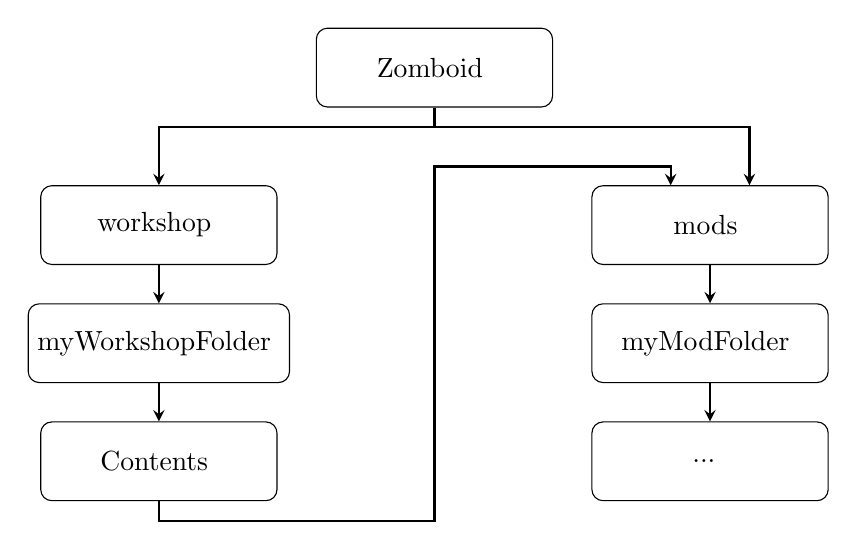
\begin{tikzpicture}[node distance=1.5cm]
    % nodes
    \node (Zomboid) [folder,align=center] { Zomboid };

    % branch left
    \node (workshop) [folder, left of=Zomboid, align=center, xshift=-2cm, yshift=-2cm] { workshop };
    \node (myWorkshopFolder) [folder, below of=workshop, align=center] { myWorkshopFolder };
    \node (Contents) [folder, below of=myWorkshopFolder, align=center] { Contents };

    % bottom
    \node (mods) [folder, right of=Zomboid, align=center, xshift=2cm, yshift=-2cm] { mods };
    \node (myModFolder) [folder, below of=mods, align=center] { myModFolder };
    \node (dotted) [folder, below of=myModFolder, align=center] { ... };

    



    % arrows

    % branch left
    \draw [arrow] (Zomboid.south) -- ([yshift=-0.25cm]Zomboid.south) -| (workshop.north);
    \draw [arrow] (workshop) -- (myWorkshopFolder);
    \draw [arrow] (myWorkshopFolder) -- (Contents);
    % \draw [arrow] (Contents) |- ([yshift=0.25cm]mods.north) -- (mods.north);

    \draw [arrow] (Contents) |- ([yshift=-0.25cm]Contents.south) -| ([yshift=-0.75cm]Zomboid.south) -| ([xshift=-0.5cm]mods.north);

    % branch right
    \draw [arrow] (Zomboid.south) -- ([yshift=-0.25cm]Zomboid.south) -| ([xshift=0.5cm]mods.north);

    % bottom
    \draw [arrow] (mods) -- (myModFolder);
    \draw [arrow] (myModFolder) -- (dotted);

    % \draw [arrow] (Zomboid.south) |- ([yshift=0.75cm,xshift=-1em]workshop.east) -| ([xshift=1cm]workshop.east) |- ([yshift=0.25cm]mods.north);
\end{tikzpicture}




\end{document}


